\documentclass[./dissertation.tex]{subfiles}
\usepackage{algorithm}
\usepackage{algpseudocode}
\begin{document}

    \contentchapter{Methodology}
    We look to discover the potential of applying components of the VAE methodology to DML systems. We test this through presenting incremental modifications to the basic DML architecture. Each modified architecture corresponds to a claim about how a specific part of the VAE training regime and loss function may be adapted to assist the performance of a DML method for a semi supervised dataset. 
    
    \begin{algorithm}
    \caption{Base DML Training Routine}\label{alg:cap}
    \hspace*{\algorithmicindent} \textbf{Input}: dataset $D$, encoder network $f$, metric loss function $l$, learning rate $\gamma$
    \begin{algorithmic}[1]
    \For{batch $X$, $Y$ in $X$}
        \State $Z = f(X)$
        \State $c = l(Z)$
        \State Calculate gradients given cost function
        \State Apply Gradients to f
    \EndFor
    \end{algorithmic}
    \hspace*{\algorithmicindent} \textbf{Output}: trained encoder $f$
    \end{algorithm}
    
    \section{DML Autoencoder}
    The first claim we look to evaluate is that the reconstruction that the autoencoder structure of the VAE and the associated reconstruction loss, helps the clustering of unlabelled points. The intutition lies in that the reconstruction loss may encourage semantic “neighborhoods” that organize points within the latent space. In other words, considering that the decoder of an autoencoder must attempt to reconstruct the original input $x$ from the latent vector $z$, it follows that $z$ must contain information about $x$. It follows that for inputs $x_{1}, x_{2}$ that are of the same class and are likely relatively similar, and thus have vectors $z_{1}, z_{2}$ that have similar values, i.e. are close to each other in the latent space. In this way, autoencoders are able to regulate the structure of the latent space like a DML model without the use of unlabelled data. \\
    
    To evaluate this claim, we construct a Metric Autoencoder architecture that incorporates reconstruction loss within the autoencoder. This architecture modifies the base DML architecture by decoding the latent vectors $z$ and calculating a reconstruction loss from the output of the decoder.. 

    \begin{algorithm}
    \caption{Base DML Autoencoder Training Routine}\label{alg:cap}
    \hspace*{\algorithmicindent} \textbf{Input}: dataset $X$, encoder network $f$, decoder network $g$, metric loss function $l$, learning rate $\gamma$, coefficient $\alpha$
    \begin{algorithmic}[1]
    \For{batch $x$ in $X$}
        \State $z = f(x)$
        \State $\hat{x} = g(z)$
        
        \State $c = l(z) + \gamma MSE(\hat{x}, x)$
        \State Calculate gradients given cost function
        \State Apply Gradients to f
    \EndFor
    \end{algorithmic}
    \hspace*{\algorithmicindent} \textbf{Output}: trained encoder $f$
    \end{algorithm}

    \section{DML with a VampPrior}
    The second claim we look to evaluate is that the structure of by positing structure onto a latent space using a prior distribution, can be used to induce bias in the latent space of a DML system. In a VAE, the latent distributions (i.e. posterior distributions) are taken as an input in the KL Divergence term of the loss function, which measures the distance between said distribution in a prior distribution. As the full VAE loss is minimized, this term encourages that the latent distributions are close to the chosen prior distribution. As discussed previously, generally the prior in a VAE is the unit gaussian, but in VAE with a VampPrior \cite{} we see that a prior distribution can be not only a mixture of several gaussians but a learnable parameter. \\
    
    We believe that adding a similar loss component which measures the KL Divergence between a prior distribution (particularly a VampPrior) and the latent distribution can help induce bias in the latent space. Specifically, if one knows that there are $n$ classes in a dataset (ex. $n = 10$ classes in MNIST), a VampPrior distribution with $n$ components may induce a bias in the latent space to make use of this information. The intuition behind this hypothesis is that a VampPrior containing $n$ gaussian components will organize the latent points into roughly $n$ clusters, where each component or cluster comes to represent a class as the VampPrior is learned. \\
    
    To evaluate this claim, we construct a DML with a VampPrior model. This architecture diverges from the base DML algorithm in three main ways. First, like a VAE, the encoder function $f$ does not map an input $x$ to a latent point but to a latent distribution, paramaterized by mean $\mu$ and variance $\sigma$. From there, a latent point $z$ is sampled from $N(\mu, \sigma)$. Taking this step from the VAE is necessary so that KL Divergence can be computed between the posterior distributions $N(\mu, \sigma)$ and the VampPrior. Second, as in VAE with a VampPrior, we will pass pseudoinputs through the encoder to construct the VampPrior distribution. The process is discussed in further detail in the VAE with a VampPrior section. Third, we will be adding the (weighted) KL Divergence loss to metric learning loss to compute the loss of the model. 
  
    \begin{algorithm}
    \caption{DML with a VampPrior Training Routine}\label{alg:cap}
    \hspace*{\algorithmicindent} \textbf{Input}: dataset $X$, encoder network $f$, metric loss function $l$, learning rate $\alpha$, coefficient $\gamma$
    \begin{algorithmic}[1]
    \For{batch $x$ in $X$}
        \State $z = f(x)$
        \State $\hat{x} = g(z)$
        \State Psuedoinput VampPrior Stuff
        \State $c = l(z) + $ VampPrior Term
        \State Calculate gradients given cost function
        \State Apply Gradients to f
    \EndFor
    \end{algorithmic}
    \hspace*{\algorithmicindent} \textbf{Output}: trained encoder $f$
    \end{algorithm}  
    
    \section{DML VAE}
    - We just use the training routine of the VAE but add the metric loss to the loss function
  
    \section{MLVAE Loss Functions}
    The third claim is that performing DML on the latent space of the VAE so that the DML task can be jointly optimized with the VAE to incorporate unlabelled data may help produce better representations. In a sense, this claim is a composite of the previous two claims, as the VAE loss function can be thought of as a weighted sum between reconstruction error and KL Divergence between the prior and posterior. However, the first two claims are likely not independent. Regardless, performing DML on the latent space of the VAE while the DML task is jointly optimized with the VAE may improve clustering quality in semi-supervised datasets as it is clear the VAE is capable of clustering unlabelled data and DML is capable of clustering labelled data. \\
    
    To evaluate this claim, we implement a DML VAE which performs DML on the latent space of a VAE, such that the DML and VAE loss functions are jointly optimized. In the DML VAE implementaiton, the training routine is very similar to the VAE (we specifically use a VAE with VampPrior). However, a metric loss is calculated with the labelled portion of a batch of embeddings $Z_{labelled}$ and added to the overall loss. \\
    
    - Other Implementation quirks: how we need to adjust training routine bc metric losses need greater batch sizes than vae loss, etc.
    \section{Evaluation of Latent Space}
    We will evaluate the results by running each model on a test partition of data. We then take the latent points $Z$ generated by the model and the corresponding labels $Y$. Three classifiers (sklearn's implementation of RandomForest, MLP, and kNN) each output predicted labels $\hat{Y}$ for the latent points. We finally measure the quality of the predicted labels $\hat{Y}$ using the Mutual Information Score (which appears to be used in the literature for this context) and accuracy (which is still helpful but is also more interpretable). The performance of a classifier on the latent points intuitively can be used as a measure of quality of clustering.


    \begin{figure}[h]
        \centering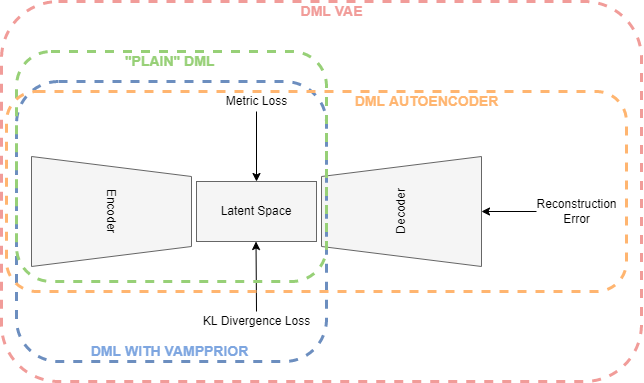
\includegraphics[width=0.5\textwidth]{figures/DML_Arcs.drawio.png}
        \caption{Comparison of Modified DML Architectures Presented}
        \label{Triplet Loss Diagram}
    \end{figure}

    
\end{document}
